\input{../preamble.tex}

\SetDate[10/03/2026]

\begin{document}
\pagestyle{fancy}
\fancyhead[L]{Seconde}
\fancyhead[C]{\textbf{Fonctions affines}}
\fancyhead[R]{\today}

\subsection*{Automatismes}


\exemulticols{}{
	Donner le domaine $\D$ du repère ci-contre.
	Calculer $4$ points appartenant aux courbes $\C_f$ et $\C_g$ et les esquisser dans le repère.
	\setlength{\columnseprule}{1pt} 
	\begin{multicols}{2}
		$f(x) = 2x + 1$
		
		\vspace{2cm}\,
		
		\columnbreak
		
		$g(x) = 2 - x$
	\end{multicols}
	
	Quel $x\in\D$ vérifie $f(x) = g(x)$ ?
	
	\vfill\,
}{

	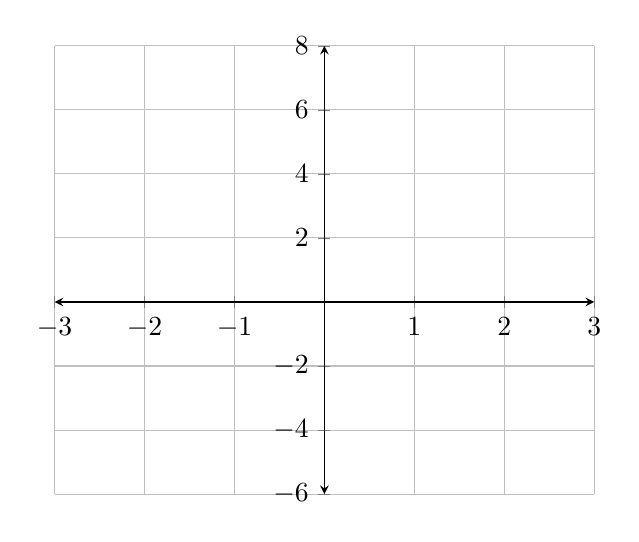
\begin{tikzpicture}[>=stealth, scale=1]
		\begin{axis}[xmin = -3, xmax=3, ymin=-6, ymax=8, axis x line=middle, axis y line=middle, axis line style=<->, xlabel={}, ylabel={}, xtick = {-3, ..., 3}, ytick = {-10, -8, ..., 8, 10}, grid=both]
		\end{axis}
	\end{tikzpicture}


}{exe:Cf-affine}{
	Un point de de la courbe représentative de $f$ prend la forme $(x ; f(x))$, où $x$ fait partie du domaine d'étude.
	
	Pour chaque fonction, les points de sa courbe représentative sont alignés.
	La courbe d'une fonction affine est en fait une droite.
	
	Les courbes représentatives sont données ci-dessous.
	\begin{center}
	\begin{tikzpicture}[>=stealth, scale=1]
		\begin{axis}[xmin = -3, xmax=3, ymin=-6, ymax=8, axis x line=middle, axis y line=middle, axis line style=<->, xlabel={}, ylabel={}, xtick = {-3, ..., 3}, ytick = {-10, -8, ..., 8, 10}, grid=both]
		
			\addplot[BLUE_E, thick, domain =-3:3, samples=2] {1+2*x}  node[pos=.2, below right] {$\mathcal{C}_f$};
			\addplot[RED_E, thick, domain =-3:3, samples=2] {2-x}  node[pos=.2, above] {$\mathcal{C}_g$};
		
			
		\end{axis}
	\end{tikzpicture}
	\end{center}

}


\exe{}{
	Pour chaque droite ci-dessous, donner 2 points lui appartenant dont un d'abscisse nulle.
	\begin{center}
	\newcommand{\scale}{1.095}
	\begin{tikzpicture}[>=stealth, scale=\scale]
	\begin{axis}[xmin = -10, xmax=10, ymin=-10, ymax=10, axis x line=middle, axis y line=middle, axis line style=<->, xlabel={}, ylabel={}, xtick = {-10, -8, ..., 8, 10}, ytick = {-10, -8, ..., 8, 10}, grid=both]
	
		\addplot[RED_E, thick, domain =-9:9, samples=2] {-x}  node[pos=.9, above=6pt] {$(\mathcal{C}_f)$};
		\addplot[RED_E, thick, dotted, domain =-10:-9, samples=2] {-x} ;
		\addplot[RED_E, thick, dotted, domain =9:10, samples=2] {-x};
	
	
		\addplot[GREEN_E, thick, domain =-9:9, samples=2] {x/2+1}  node[pos=.9, below=6pt] {$(\mathcal{C}_g)$};
		\addplot[GREEN_E, thick, dotted, domain =-10:-9, samples=2] {x/2+1} ;
		\addplot[GREEN_E, thick, dotted, domain =9:10, samples=2] {x/2+1};
	
	
		\addplot[BLUE_E, thick, domain =-9:9, samples=2] {7}  node[pos=.7, above] {$(\mathcal{C}_h)$};
		\addplot[BLUE_E, thick, dotted, domain =-10:-9, samples=2] {7} ;
		\addplot[BLUE_E, thick, dotted, domain =9:10, samples=2] {7};
	\end{axis}
	\end{tikzpicture}
	\begin{tikzpicture}[>=stealth, scale=\scale]
	\begin{axis}[xmin = -10, xmax=10, ymin=-10, ymax=10, axis x line=middle, axis y line=middle, axis line style=<->, xlabel={}, ylabel={}, xtick = {-10, -8, ..., 8, 10}, ytick = {-10, -8, ..., 8, 10}, grid=both]
	
		\addplot[RED_E, thick, domain =-9:9, samples=2] {-x/3 + 1}  node[pos=.9, below=5pt] {$(\mathcal{C}_F)$};
		\addplot[RED_E, thick, dotted, domain =-10:-9, samples=2] {-x/3 + 1} ;
		\addplot[RED_E, thick, dotted, domain =9:10, samples=2] {-x/3 + 1};
	
	
		\addplot[GREEN_E, thick, domain =-5:7, samples=2] {3*x/2-2}  node[pos=.2, left] {$(\mathcal{C}_G)$};
		\addplot[GREEN_E, thick, dotted, domain =-6:-5, samples=2] {3*x/2-2} ;
		\addplot[GREEN_E, thick, dotted, domain =7:8, samples=2] {3*x/2-2};
	
	
		\addplot[BLUE_E, thick, domain =-9:9, samples=2] {-x/6 + 5}  node[pos=.2, above] {$(\mathcal{C}_H)$};
		\addplot[BLUE_E, thick, dotted, domain =-10:-9, samples=2] {-x/6 + 5} ;
		\addplot[BLUE_E, thick, dotted, domain =9:10, samples=2] {-x/6 + 5};
	\end{axis}
	\end{tikzpicture}
	\end{center}
	
	%\begin{enumerate}
		%\item Pour chacune des droites ci-dessus, donner $2$ points lui appartenant, dont un d'abscisse nulle.
		%\item En déduire l'ordonnée à l'origine $b$ de chacune des fonctions affines $f, g, h, F, G,$ et $H$.
		%\item Donner le signe (strictement positif, strictement négatif, ou nul) du coefficient directeur $a$ de chacune des fonctions affines $f, g, h, F, G,$ et $H$.
	%\end{enumerate}
}{exe:lecture-points}{
	\begin{enumerate}
		\item[$f$:] 
		\begin{enumerate}[label=\arabic*.]
			\item $(0;0)$ et $(2;-2)$ appartiennent à $\C_f$.
			\item On en déduit que $f(x) = ax + 0 = ax$ pour un certain paramètre $a$ encore indéterminé.
		\end{enumerate}
		\item[$g$:] 
		\begin{enumerate}[label=\arabic*.]
			\item $(0;1)$ et $(-2; 0)$ appartiennent à $\C_f$.
			\item On en déduit que $f(x) = ax + 1$ pour un certain paramètre $a$ encore indéterminé.
		\end{enumerate}
		\item[$h$:] 
		\begin{enumerate}[label=\arabic*.]
			\item $(0;7)$ et $(6;7)$ appartiennent à $\C_f$.
			\item On en déduit que $f(x) = ax + 7$ pour un certain paramètre $a$ encore indéterminé. Comme $h$ est constante, on peut deviner que $a=0$...
		\end{enumerate}
		\item[$F$:] 
		\begin{enumerate}[label=\arabic*.]
			\item $(0;1)$ et $(3;0)$ appartiennent à $\C_f$.
			\item On en déduit que $f(x) = ax + 1$ pour un certain paramètre $a$ encore indéterminé.
		\end{enumerate}
		\item[$G$:] 
		\begin{enumerate}[label=\arabic*.]
			\item $(0;-2)$ et $(-4;-8)$ appartiennent à $\C_f$.
			\item On en déduit que $f(x) = ax -2$ pour un certain paramètre $a$ encore indéterminé.
		\end{enumerate}
		\item[$H$:] 
		\begin{enumerate}[label=\arabic*.]
			\item $(0;5)$ et $(6;4)$ appartiennent à $\C_f$.
			\item On en déduit que $f(x) = ax +5$ pour un certain paramètre $a$ encore indéterminé.
		\end{enumerate}
	\end{enumerate}
}

%^\vspace{-10pt}
\subsection*{Exercices}


\exe{, difficulty=1}{
		Lire graphiquement un vecteur directeur de chaque droite de l'exercice \ref{exe:lecture-points} et en déduire le coefficient directeur $a$ de la fonction affine associée.
}{exe:coeff-dir}{
	On calcule le coefficient directeur à l'aide des paires de points qu'on a donné à l'exercice \ref{exe:lecture-points}.

	\begin{enumerate}
		\item[$f$:] 
			Les points $(0;0)$ et $(2;-2)$ appartiennent à $\C_f$.
			Donc 
				\[ a = \dfrac{-2 - 0}{2-0} = -1, \]
			et $f(x) = -x$.
		\item[$g$:] 
			Les points $(0;1)$ et $(-2;0)$ appartiennent à $\C_g$.
			Donc 
				\[ a = \dfrac{0 - 1}{-2-0} = \dfrac12, \]
			et $g(x) = \dfrac12 x + 1$.
		\item[$h$:] 
			Les points $(0;7)$ et $(6;7)$ appartiennent à $\C_h$.
			Donc 
				\[ a = \dfrac{7-7}{6-0} = 0, \]
			et $h(x) = 7$, une fonction constante.
		\item[$F$:] 
			Les points $(0;1)$ et $(3;0)$ appartiennent à $\C_F$.
			Donc 
				\[ a = \dfrac{0-1}{3-0} = -\dfrac13, \]
			et $F(x) = -\dfrac13 x + 1$, une fonction constante.
		\item[$G$:] 
			Les points $(0;-2)$ et $(-4;-8)$ appartiennent à $\C_G$.
			Donc 
				\[ a = \dfrac{-8-(-2)}{-4-0} = \dfrac{-6}{-4} = \dfrac32, \]
			et $G(x) = \dfrac32 x - 2$, une fonction constante.
		\item[$H$:] 
			Les points $(0;5)$ et $(6;4)$ appartiennent à $\C_H$.
			Donc 
				\[ a = \dfrac{4-5}{6-0} = \dfrac{-1}{6}, \]
			et $H(x) = -\dfrac16 x + 5$, une fonction constante.
	\end{enumerate}
}

\exe{}{
	Pour chaque fonction affine sur $\R$ suivante, déterminer son coefficient directeur $a$ et son ordonnée à l'origine $b$.
	\begin{multicols}{2}
	\begin{enumerate}
		\item $f(x) = 2x + 1$
		\item $f(x) = 1 + 2x$
		\item $f(x) = - x$
		\item $f(x) = -42$
		\item $f(x) = \sqrt{3} \cdot x + 2$
		\item $f(x) = 2 - \dfrac{\pi}{6}x$
		\item $f(x) = 1 - x$
		\item $f(x) = 0$
	\end{enumerate}
	\end{multicols}
}{exe:parametres-affines}{
	On a en général
		\[ f(x) = a \cdot x + b. \]
	On lit donc le coefficient directeur $a$ comme le nombre réel qui multiplie $x$.
	Les cas particuliers suivants sont importants.
	\begin{itemize}
		\item 
		Si $x$ n'apparaît pas en premier, il est possible d'échanger les termes en gardant en tête que le signe s'accroche à la valeur de droite. Par exemple, $3-2x = -2x + 3$.
		\item
		Si $x$ n'apparaît pas, $f$ est constante, et $a$ est nul.
		\item
		Si aucun nombre n'apparait devant $x$, on peut le créer en écrivant $x = (1) \cdot x$.
		\item
		Idem pour $-x = (-1) \cdot x$ : on change d'écriture pour mettre en exergue le coefficient qui multiplie $x$.
		\item
		On lit l'ordonnée à l'origine $b$ comme la partie constante de la fonction.
		Si rien n'apparait, on peut la créer en ajoutant $0$. Par exemple, $2x = 2x+0$.
	\end{itemize}
	
	Les relations
		\begin{align*}
			f(0) = b && \et && f(1)-f(0) = a
		\end{align*}
	permettent aussi de calculer $a$ et $b$ en deux évaluations de $f$.

	\begin{multicols}{4}
	\begin{enumerate}
		\item 
			$
				a = 2	$ et $ b = 1
			$
		\item
			$
				a = 2	$ et $ b = 1
			$
		\item 
			$
				a = -1	$ et $ b = 0
			$
		\item 
			$
				a = 0	$ et $ b = -42
			$
		\item 
			$
				a = \sqrt{3}	$ et $ b = 2
			$
		\item 
			$
				a = -\frac{\pi}{6}$ et $ b = 2
			$
		\item 
			$
				a = -1	$ et $ b = 1
			$
		\item
			$
				a = 0	$ et $ b = 0
			$
	\end{enumerate}
	\end{multicols}
}




\exemulticols{, difficulty=1}{
	Soient $f(x) = ax+b$ et $g(x) = a'x+b'$ deux fonctions affines données graphiquement pour $x\in[3,2 ; 3,7]$ ci-contre.
	
	Déterminer les paramètres $a, b, a',$ et $b'$.
	\vfill\,
}{
	\begin{center}
	\begin{tikzpicture}[>=stealth, scale=.8]
	\begin{axis}[xmin = 3.2, xmax=3.7, ymin=5, ymax=7, axis x line=middle, axis y line=middle, axis line style=->, xtick distance=.1, ytick distance = 1,  enlargelimits=.1, grid=both, clip=true, minor x tick num = 1, minor y tick num = 3, x=500pt]
		
		% Cf
		\addplot[BLUE_E, very thick, domain =3.2:3.7, samples=2] {-1+2*x}  node[pos = .9, above left] {$\C_f$};
		\addplot[BLUE_E, very thick, dashed, domain =3.1:3.2, samples=2] {-1+2*x} ;
		\addplot[BLUE_E, very thick, dashed, domain =3.7:3.8, samples=2] {-1+2*x};
		
		% Cg
		\addplot[RED_E, very thick, domain =3.2:3.7, samples=2] {13-2*x}  node[pos = .9, below left] {$\C_g$};
		\addplot[RED_E, very thick, dashed, domain =3.1:3.2, samples=2] {13-2*x};
		\addplot[RED_E, very thick, dashed, domain =3.7:3.8, samples=2] {13-2*x};
	\end{axis}
	\end{tikzpicture}
	\end{center}
}{exe:extrapolation-graphique1}{
	Notons $f(x) = ax + b$ la fonction affine.
	On utilise le lemme du cours qui dit que $(0 ; b) \in \C_f$ pour déduire que $b=-1$ car $(0; -1) \in \C_f$.
	
	On utilise enfin le théorème du cours qui implique que, en choisissant $A(-0,5 ; -3,5)$ et $B(0,5;1,5)$,
		\[ a = \dfrac{y_B - y_A}{x_B - x_A} = \dfrac{1,5 - (-3,5)}{0,5 - (-0,5)} = \dfrac41 = 4. \]
	Remarquons que, quand $x$ augmente de $1$, $f(x)$ augmente de $4$, le coefficient directeur.
	De plus, l'ordre des points n'a en fait pas d'importance : on aurait pû choisir $B(-0,5 ; -3,5)$ et $A(0,5;1,5)$ pour trouver le même coefficient directeur.
	
	On conclut que 
		\[ f(x) = 4x - 1. \]
}



\exe{, difficulty=1}{
	Pour chacune des paires de points $A, B$ suivantes, calculer les paramètres ($a$ et $b$) de l'unique fonction affine $f$ telle que $A$ et $B$ appartiennent à $\C_f$.
	
	\begin{multicols}{2}
	\begin{enumerate}
		\item $A(1;2), B(4;-4)$.
		\item $A(2;8), B(4;7)$.
		\item $A(4;7), B(2;8)$.
		\item $A(-3; -3), B(-2; -1)$.
		\item $A(2;5), B(-10; 5)$.
		\item $A(-3;4), B(12;-11)$.
	\end{enumerate}
	\end{multicols}

}{exe:inter-extrapolation}{
	On utilise la convention $a, b \in \R$ pour désigner respectivement le coefficient directeur et l'ordonnée à l'origine de la fonction affine $f$.
	$f(x) = ax+b$ pour tout $x\in\R$.

	\begin{enumerate}
		\item 
		D'après le cours,
		\begin{align*}
			a = \dfrac{y_A - y_B}{x_A - x_B}, && y_A = f(x_A).
		\end{align*}
		Par suite,
		\begin{align*}
			a = \dfrac{2 - (-4)}{1 - 4} = -2, && 2 = -2\cdot(1)+b \iff b=4.
		\end{align*}
				
		\item 
		\begin{align*}
			a = \dfrac{8-7}{2-4} = -\dfrac12, && 8 = -\dfrac12\cdot(2)+b \iff b=9.
		\end{align*}
			
		Graphiquement : le point $A$ est à gauche du point $B$ car son abscisse est plus petite et est plus haut que le point $B$ car son ordonnée est plus grande. 
			La fonction $f$ doit donc être décroissante, ce qu'on a bien trouvé car $a<0$.
		\item
		\begin{align*}
			a = \dfrac{7-8}{4-2} = -\dfrac12, && b = 7 = -\dfrac12\cdot(4) + b \iff b = 9.
		\end{align*}
			
		Les formules ne dépendent bien sûr pas de l'ordre de $A$ et $B$ car la droite $(AB)$ est égale à la droite $(BA)$.
					
		\item
		\begin{align*}
			a = \dfrac{-3-(-1)}{-3-(-2)} = 2, && -3 = 2\cdot(-3) + b \iff b=3.
		\end{align*}
			
		\item
		\begin{align*}
			a = \dfrac{5-5}{2-(-10)} = 0, && 5 = 0\cdot(2) + b \iff b=5.
		\end{align*}
		
		Graphiquement : les deux points sont à la même hauteur car leurs abscisses sont égales.
		La droite $(AB)$ est donc horizontale, d'où $a=0$, et sa hauteur est celle des points, d'où $b=5$.
			
		\item $A(-3;4), B(12;-11)$.
		\begin{align*}
			a = \dfrac{4-(-11)}{-3-12} = -1, && 4 = -1\cdot(-3) + b \iff b = 1.
		\end{align*}
		
		Vérification : on vérifie que $A$ et $B$ vérifient bien l'équation $y=f(x) = -x +1$ en remplaçant les valeurs par les coordonnées.
		Ainsi pour $A$ on a bien $y=4$ à gauche, et $f(-3) = -(-3) + 1 = 4$ à droite.
		Pour $B$, on a $y=-11$ à gauche, et $f(12) = -12 + 1 = -11$ à droite.
	\end{enumerate}
}



\exe{, difficulty=1}{
	Pour chaque paire $(f, g)$ de fonctions affines sur $\R$, calculer l'intersection $\C_f \cap \C_g$.
	
	\begin{multicols}{2}
	\begin{enumerate}
		\item $f(x) = 2x + 1, g(x) = -x+1$.
		\item $f(x) = -x + 1, g(x) = 2x + 1$.
		\item $f(x) = 3+7x, g(x) = 2$.
		\item $f(x) = 9-2x, g(x) = 17-x$.
		\item $f(x) = 2x+1, g(x) = 2x+1$.
		\item $f(x) = 2x+1, g(x) = 2x+2$.
	\end{enumerate}
	\end{multicols}
}{exe:affine-intersection}{

	\begin{enumerate}
		\item $f(x) = 2x + 1, g(x) = -x+1$ .
			On cherche un point $P(x_P, y_P)$ vérifiant les deux équations
				\begin{align*}
					y_P = f(x_P) && \text{ et } && y_P = g(x_P)
				\end{align*}
			Comme bien sûr $y_P = y_P$, on peut résoudre l'équation
				\[ f(x_P) = g(x_P) \]
			pour trouver $x_P$.
			Ici, on pose calmement
				\begin{align*}
					f(x_P) &= g(x_P) \\
					2x_P + 1 &= -x_P + 1 \\
					3x_P &= 0 \\
					x_P &= 0,
				\end{align*}
			ce qui nous fournit $x_P = 0$.
			Reste plus qu'à utiliser que $y_P = f(x_P) = g(x_P)$ pour calculer $y_P$.
			
			D'une part, 
				\[ f(x_P) = f(0) = 2\cdot0 + 1 = 1. \]
			D'autre part, on aurait pû calculer
				\[ g(x_P) = g(0) = -0 + 1 = 1. \]
			Rien de surprenant à ce qu'on trouve la même valeur $y_P = 1$, car $x_P$ a été trouvé vérifiant $f(x_P) = g(x_P)$.
			
			En conclusion, $\C_f \cap \C_g = \{ (0;1) \}$.
			
		\item 
			Similairement,
			\begin{align*}
				f(x_P) &= g(x_P) \\
				-x_P + 1 & = 2x_P + 1 \\
				x_P &= 0,
			\end{align*}
			et $y_P = f(0) = 1$.
			Sans surprise, $(0;1)$ est à nouveau le point d'intersection de $\C_f$ et de $\C_g$ car se sont les mêmes fonctions que ci-dessus mais échangées.
		
		\item 
			Similairement,
			\begin{align*}
				f(x_P) &= g(x_P) \\
				3 + 7x_P & = 2 \\
				7x_P &= -1 \\
				x_P &= \dfrac{-1}7,
			\end{align*}
			\[
				y_P = f(x_P) = 3+7\cdot \dfrac{-1}7  = 2.
			\]
			Il aurait été encore plus facile de calculer $g(x_P) = 2$ à la place !
			
			En conclusion, $\C_f \cap \C_g = \left\{ \left(-\dfrac72 ; 2\right) \right\}$.
		
		\item
			Similairement,
			\begin{align*}
				f(x_P) &= g(x_P) \\
				9-2x_P & = 17-x_P \\
				-8 &= x_P,
			\end{align*}
			\[
				y_P = f(x_P) = 9-2 \cdot(-8) = 25.
			\]
		
			En conclusion, $\C_f \cap \C_g = \left\{ (-8;25) \right\}$.
		
		\item 			
		Similairement,
			\begin{align*}
				f(x_P) &= g(x_P) \\
				2x_P + 1 & = 2x_P + 1 \\
				0 &= 0,
			\end{align*}
			cette équation étant évidemment vraie, tous les $x_P \in \R$ vérifient l'équation.
			\[
				y_P = f(x_P) = 2x_P + 1.
			\]
			N'importe quel $(x_P ; 2x_P+1) \in \R$ appartient donc à l'intersection des droites.
			
			En conclusion, $\C_f \cap \C_g = \bigset{ (x_P ; 2x_P+1) \text{ tq. } x_P \in \R } = \bigset{ (x_P ; y_P) \text{ tq. } y_P = 2x_P + 1 } = \C_f = \C_g$.
			Il n'est pas surprenant qu'on trouve que toute la droite appartienne à l'intersection, car $f$ et $g$ sont identiques : tous les points de la droite $\C_f$ sont des points d'intersection.
		
		
		\item 
			Similairement,
			\begin{align*}
				f(x_P) &= g(x_P) \\
				2x_P + 1 & = 2x_P + 2 \\
				1 &= 2,
			\end{align*}
			cette équation étant évidemment fausse, aucun $x_P \in \R$ ne vérifie l'équation.
			
			En conclusion, $\C_f \cap \C_g = \emptyset$, l'ensemble vide.
			En fait, les droites $\C_f$ et $\C_g$ sont parallèles car elles ont le même coefficient directeur $2$.
			Or les droites ne sont pas égales car leurs ordonnées à l'origine sont différentes, donc il n'y a aucun point d'intersection.
	\end{enumerate}

}

\exe{, difficulty=1}{
	Pour chacun des couples de point $P$ et fonction affine $f$ sur $\R$, trouver la fonction affine $g$ telle que $\C_f$ et $\C_g$ soient parallèles et que $P \in \C_g$.
	
	
	\begin{multicols}{2}
	\begin{enumerate}
		\item $P=(1;2)$ et $f(x) = 2x+1$.
		\item $P= (-2; 4)$ et $f(x) = 7-x$.
		\item $P=(-4^{12};-1,7)$ et $f(x) = 1600$.
		\item $P=(21;-50,5)$ et $f(x) = -3x + 5$.
	\end{enumerate}
	\end{multicols}
}{exe:affine-parallelisme}{
	On pose $a, b\in\R$ les paramètres de la fonction affine $g(x)=ax+b$, $x\in\R$.
	\begin{enumerate}
		\item 
			L'information de parallélisme donne immédiatement $a=2$.
			D'où $g(x) = 2x+b$ pour tout $x\in\R$.
			
			Reste à trouver $b$ avec l'information d'appartenance.
			Celle-ci est équivalente à la contrainte
				\begin{align*}
					2 &= g(1) \\
					2 &= 2\cdot1 + b \\
					b &= 0
				\end{align*}
			D'où $g(x) = 2x$ ($x\in\R$) est la fonction affine recherchée.
		
		
		\item 
			L'information de parallélisme donne immédiatement $a=-1$.
			D'où $g(x) = -x+b$ pour tout $x\in\R$.
			
			Reste à trouver $b$ avec l'information d'appartenance.
			Celle-ci est équivalente à la contrainte
				\begin{align*}
					2 &= g(1) \\
					2 &= -1 + b \\
					b &= 3
				\end{align*}
			D'où $g(x) = -x+3$ ($x\in\R$) est la fonction affine recherchée.
			
		\item 
			L'information de parallélisme donne immédiatement $a=0$.
			D'où $g(x) =b$ pour tout $x\in\R$.
			
			Reste à trouver $b$ avec l'information d'appartenance.
			Celle-ci est équivalente à la contrainte
				\begin{align*}
					2 &= g(1) \\
					2 &=  b
				\end{align*}
			D'où $g(x) = 2$ ($x\in\R$) est la fonction affine recherchée.
			
		\item 
			L'information de parallélisme donne immédiatement $a=-3$.
			D'où $g(x) = -3x+b$ pour tout $x\in\R$.
			
			Reste à trouver $b$ avec l'information d'appartenance.
			Celle-ci est équivalente à la contrainte
				\begin{align*}
					2 &= g(1) \\
					2 &= -3\cdot1 + b \\
					b &= 5
				\end{align*}
			D'où $g(x) = -3x+5$ ($x\in\R$) est la fonction affine recherchée.
	\end{enumerate}

}

\subsection*{Approfondissements}



\exe{, difficulty=2}{
	Considérons les points $O(0;0)$ et $P(3 ; 1)$ et $(d)$ la médiatrice du segment $[OP]$ : ce sont tous les points $M(x;y)$ à équidistance de $O$ et $P$.
	
	Montrer que $x$ et $y$ sont liés par la relation 
		$ y = -3x + 5. $
}{exe:médiatrice}{
	À rendre pour possibilité de points bonus à la prochaine évaluation.
	Ni correction ni points ne seront attribués à un travail suspect ou ne démontrant pas une bonne compréhension de l'exercice.
	
	
%	La contrainte d'équidistance s'exprime et est équivalente aux équations suivantes.
%		\begin{align*}
%			\norm{M-O}^2 &= \norm{M - P}^2 \\
%			x^2 + y^2 &= (x-3)^2 + (y-1)^2 \\
%			x^2 + y^2 &= x^2 - 6x + 9 + y^2 - 2y + 1 \\
%			2y &= -6x + 10 \\
%			y &= -3x + 5
%		\end{align*}
}


\exe{, difficulty=3}{
	Considérons une fonction quadratique 
		$ f(x) = ax^2 + bx + c, $
	où $a, b, c\in\R$ sont trois paramètres réels.
	Supposons qu'on connaisse deux \emph{racines} distinctes de $f$, c'est-à-dire qu'on connaisse $\alpha, \beta\in\R$ tels que $\alpha\neq\beta$ et
		\[ f(\alpha) = f(\beta) = 0. \]
	\begin{enumerate}
		\item Montrer que la fonction $g(x) = f(x) - a (x-\alpha)(x-\beta)$ est affine.
			%\[ g(x) = f(x) - a (x-\alpha)(x-\beta) \qquad \text{ pour tout } x\in\R. \]
		\item Montrer que $g$ admet deux racines distinctes.
		\item En déduire que $g$ est constamment nulle et donc que
%			\begin{align*}
%				\alpha+\beta = -\dfrac{b}a, && \alpha\cdot\beta = \dfrac{c}a, && f(x) = a (x-\alpha)(x-\beta)  \qquad \text{ pour tout } x\in\R.
%			\end{align*}
			\[ f(x) = a (x-\alpha)(x-\beta)  \qquad \text{ pour tout } x\in\R.\]
		On dit alors que $f$ se \emph{scinde} en produit affine.
	\end{enumerate}
}{exe:thm-fond-alg-2}{
	À rendre pour possibilité de points bonus à la prochaine évaluation.
	Ni correction ni points ne seront attribués à un travail suspect ou ne démontrant pas une bonne compréhension de l'exercice.
	
	\underline{Discussion}
	
	Il s'avère qu'un résultat plus général est atteignable : si $\alpha\in\R$ est une racine d'un polynôme\footnote{Une fonction de la forme $f(x) = a_n x^n + a_{n-1}x^{n-1} + \hdots + a_1 x + a_0$ dont les $a_i$ sont des coefficients fixés.} $f$ de n'importe quel degré\footnote{La plus haute puissance de $x$ : le degré de $2x^2 -3x^4 + 12$ est 4.}, alors on a nécessairement $f(x) = (x-\alpha)\cdot g(x)$ pour un polynôme $g$.
	La démonstration se base sur la division euclidienne dans les polynômes :
	pour n'importe quels polynômes $f, g$, il existe deux polynômes $q, r$ vérifiants 
		\[ f = qg + r, \]
	avec le degré de $r$ strictement inférieur au degré de $g$.
	
	Dans notre cas, il doit exister un polynôme $q$ et une constante $r$ tels que $f(x) = q(x)\cdot(x-\alpha) + r$.
	En évaluant en $x=\alpha$, on obtient que $r=0$.
	
	En répétant le processus, tout polynôme de degré $n$ admettant $n$ racines se scinde en produit affine.
	En revanche, tous les polynômes n'admettent pas de racines réelles !
	C'est le cas du polynôme $x^2 + 1$ qui, lui, ne peut pas se scinder comme $(x-\alpha)(x-\beta)$ car $\alpha$ et $\beta$ seraient alors deux racines de $x^2 + 1$.
	 Or $x^2 + 1$ ne s'annule jamais, le carré étant toujours positif !
	 
	Supposons désormais qu'on ait un ensemble de nombres contenant $\R$ ainsi qu'un nouveau « nombre », racine hypothétique de $x^2 + 1$ ; est-ce que tous les polynômes se scindent dans cet ensemble\footnote{Il faut aussi qu'on puisse ajouter et multiplier dans cet ensemble tout en restant à l'intérieur ; c'est la \emph{stabilité}.} ? 
	Le \emph{théorème fondamental de l'algèbre} répond positivement à cette question.
	Ce nombre hypothétique est nommé $i$, dont la construction formelle utilise, notamment, la division euclidienne des polynômes !
}


%%%%%%%%%%%

\newpage
\fancyhead[C]{\textbf{Solutions}}
\shipoutAnswer

\end{document}
